\documentclass[]{article}
\newcommand{\FileDepth}{../..}
\usepackage[a4paper, total={15cm,23cm}]{geometry}
\usepackage[T1]{fontenc}
\usepackage{textcomp}%Not strictly necessary, but gives \textmu command for "micro."
\usepackage{fancyhdr}
\usepackage{amsmath}
\usepackage{amssymb}
\usepackage{graphicx}
\usepackage{xcolor}
\usepackage{tikz}
\usetikzlibrary{calc}
%opening
\newcommand{\SecType}{X}
\newcommand{\Week}{X}
\title{Crate Brick Box Car FBDs}
\author{Benjamin Bauml}
\date{Winter 2025}
\pagestyle{fancy}
\rhead{PH 211}
\chead{Winter 2025}
\lhead{Week \Week}

% For Assignment, leave Purpose as 1. For Worksheet, set to 2. For Student Solution, set to 3. For Teacher Solution, set to 4.
% If you want keep the pieces from being called manually, set DefOnly to 0.
\newcommand{\Purpose}{4}
\newcommand{\DefOnly}{1}

% Version 2024-06-14
% Changes
% 2024-02-21 Added xstring package to enable smooth implementation of new \ModePage command.
% 2024-04-27 Set up to split activities and formatting aspects into separate files. Removed dependence on xcomment. Added an automatic counter to number the activities in a problem set.
% 2024-05-19 Revised old format for \TeachingTips command, which did not support \DefOnly.
% 2024-06-14 Added Repurpose environment to allow mixing of different purpose levels in the same document.
\usepackage{tcolorbox}
\usepackage{xstring}
% You will want the following four lines in your document (the last two uncommented):
% For Assignment, leave Purpose as 1. For Worksheet, set to 2. For Student Solution, set to 3. For Teacher Solution, set to 4.
% If you want keep the pieces from being called manually, set DefOnly to 0.
%\newcommand{\Purpose}{4}
%\newcommand{\DefOnly}{1}
\newcommand{\Exclusion}{0}
\newcommand{\PageTurn}{0}
\newcommand{\GrayProb}{0}
\newcommand{\Tipsy}{0}

% Assignment
\if\Purpose1
\renewcommand{\Exclusion}{1}
\fi
% Worksheet
\if\Purpose2
\renewcommand{\Exclusion}{1}
\renewcommand{\PageTurn}{1}
\fi
% Student Solution
\if\Purpose3
\renewcommand{\PageTurn}{1}
\renewcommand{\GrayProb}{1}
\fi
% Teaching Copy
\if\Purpose4
\renewcommand{\PageTurn}{1}
\renewcommand{\GrayProb}{1}
\renewcommand{\Tipsy}{1}
\fi

\newenvironment{Repurpose}[1]{
\renewcommand{\Purpose}{#1}
\renewcommand{\Exclusion}{0}
\renewcommand{\PageTurn}{0}
\renewcommand{\GrayProb}{0}
\renewcommand{\Tipsy}{0}
% Assignment
\if\Purpose1
\renewcommand{\Exclusion}{1}
\fi
% Worksheet
\if\Purpose2
\renewcommand{\Exclusion}{1}
\renewcommand{\PageTurn}{1}
\fi
% Student Solution
\if\Purpose3
\renewcommand{\PageTurn}{1}
\renewcommand{\GrayProb}{1}
\fi
% Teaching Copy
\if\Purpose4
\renewcommand{\PageTurn}{1}
\renewcommand{\GrayProb}{1}
\renewcommand{\Tipsy}{1}
\fi
}{}

\def \NewQ {0}
\def \PForce {0}
\newcommand{\MaybePage}[1]{
	\def \PForce {#1}
	\if\PForce1
	\newpage
	\else
	\if\NewQ0
	\gdef \NewQ {\PageTurn}
	\else
	\newpage
	\fi
	\fi
}

\newcommand{\ModePage}[1]{
	\IfSubStr{#1}{\Purpose}{\newpage}{}
}

\newcounter{ActNumber}
\setcounter{ActNumber}{0}

\newcommand{\Problem}[4][0]{%The first argument is optional, and if it is set to 1, the \newpage will be forced. The second argument is the name of the activity, the third is the command the activity is stored as, and the fourth is the actual problem statement.
\newcommand{#3}{
\MaybePage{#1}
\addtocounter{ActNumber}{1}
\section*{\SecType\Week-\theActNumber: #2}
\if\GrayProb1
\begin{tcolorbox}[colback=lightgray,colframe=lightgray,sharp corners,boxsep=1pt,left=0pt,right=0pt,top=0pt,bottom=0pt,after skip=2pt]
\else
\begin{tcolorbox}[colback=white,colframe=white,sharp corners,boxsep=1pt,left=0pt,right=0pt,top=0pt,bottom=0pt,after skip=2pt]
\fi
#4
\end{tcolorbox}\noindent
}
\if\DefOnly0
\else
#3
\fi
}
	
\newcommand{\ProblemSub}[3][0]{%The first argument is optional, and if a string of numbers is entered into it, it will force a \newpage in any \Purpose that shows up in the string. For example, "13" would lead to the newpage being forced in modes 1 and 3. The second is the command the activity is stored as, and the third is the actual problem statement.
\newcommand{#2}{
\ModePage{#1}
\if\GrayProb1
\begin{tcolorbox}[colback=lightgray,colframe=lightgray,sharp corners,boxsep=1pt,left=0pt,right=0pt,top=0pt,bottom=0pt,after skip=2pt]
\else
\begin{tcolorbox}[colback=white,colframe=white,sharp corners,boxsep=1pt,left=0pt,right=0pt,top=0pt,bottom=0pt,after skip=2pt]
\fi
#3
\end{tcolorbox}\noindent
}
\if\DefOnly0
\else
#2
\fi
}
		
\newcommand{\Solution}[2]{%The first argument is the command the solution is stored as, and the second is the actual solution.
\newcommand{#1}{
\if\Exclusion0
#2
\fi
}
\if\DefOnly0
\else
#1
\fi
}
		
\newcommand{\ProblemFig}[2]{%The first argument is the command the figure is stored as, and the second is the actual figure.
\newcommand{#1}{
\begin{figure}[h]
#2
\end{figure}
}
\if\DefOnly0
\else
#1
\fi
}

\newcommand{\TeachingTips}[2]{%The first argument is the command the tip is stored as, and the second is the actual tip.
\newcommand{#1}{
\if\Tipsy1
\begin{tcolorbox}[colback=lightgray,colframe=black]
#2
\end{tcolorbox}
\fi
}
\if\DefOnly0
\else
#1
\fi
}

\newcommand{\FBDaxes}[3]{
	\begin{scope}[shift={(#1)},rotate=#2]
		% x-axis
		\draw[thick,->] (-2,0) -- (2,0);
		\node[anchor=west] at (2,0) {$x$};
		% y-axis
		\draw[thick,->] (0,-2) -- (0,2);
		\node[anchor=west] at (0,2) {$y$};
		\coordinate (#3) at (0,0);
	\end{scope}
}
\newcommand{\FBDvectorMA}[4]{
	\begin{scope}[shift={(#1)}]
		\coordinate (#4tip) at ({#2*cos(#3)},{#2*sin(#3)});
		\draw[ultra thick,blue,->] (#1) -- (#4tip);
	\end{scope}
}
\newcommand{\FBDvectorXY}[3]{
	\begin{scope}[shift={(#1)}]
		\coordinate (#3tip) at (#2);
		\draw[ultra thick,blue,->] (0,0) -- (#3tip);
	\end{scope}
}
\newcommand{\FBDdot}[1]{
	\filldraw[black] (#1) circle (3pt);
}
%\newcommand{\MVec}[3][0]{%Creates a momentum vector of length #3 centered at #2 and rotated #1 degrees counterclockwise.
	\begin{scope}[rotate=#1,shift={(#2)}]
		\draw[->,thick] ({-#3/2},0) -- ({#3/2},0);
	\end{scope}
}
\newcommand{\MDot}[1]{%Creates a dot at #1 to represent a zero vector.
	\filldraw (#1) circle (1pt);
}
\newcommand{\MVDRows}[2][4.5]{%Creates the rows (initial, delta, final) of a momentum vector diagram. The optional argument determines the width of the table, and defaults to a good length for three columns (two objects and the total system). The non-optional argument gives a coordinate name (not displayed) to the diagram.
	\begin{scope}
		%\draw[thick] (0,5.5) -- (0,0);
		\draw[thick] (-1,4.5) -- (#1,4.5);
		\node at (-0.5,3.75) {$\vec{p}_{i}$};
		\draw[thick] (-1,3) -- (#1,3);
		\node at (-0.5,2.25) {$\Delta\vec{p}$};
		\draw[thick] (-1,1.5) -- (#1,1.5);
		\node at (-0.5,0.75) {$\vec{p}_{f}$};
		\coordinate (#2) at (0,5);
	\end{scope}
}
\newcommand{\MVDCol}[4][0.75]{%Creates a column for an object in a momentum vector diagram. The first (non-optional) argument is the coordinate name (not displayed) of the column, while the second is the displayed column header. The first argument also names the three entries down the column. The third argument anchors the column, so it should either be the coordinate name of the MVD (for the first column) or the coordinate name of the previous column. The optional argument indicates how far the center of the column should be from the previous column's edge, and defaults to 0.75
	\begin{scope}[shift={(#4)}]
		\node at (#1,0) {#3};
		%\draw[thick] ({#1*2},0.5) -- ({#1*2},-5);
		\draw[thick] (0,0.5) -- (0,-5);
		\coordinate (#2init) at (#1,-1.25);
		\coordinate (#2delt) at (#1,-2.75);
		\coordinate (#2fin) at (#1,-4.25);
		\coordinate (#2) at ({#1*2},0);
	\end{scope}
}

\begin{document}
\maketitle

\Problem{Crate, Brick, Box, and Car FBDs}{\CrateBrickBoxCar}{
	For the following exercises, draw the situation and identify and name all the forces acting on the object. Then, using the particle model, draw a free-body diagram for the object. Include the direction of the net force $ \vec{F}_{net} $. Neglect air resistance.
}
\ProblemSub{\Crate}{
	(a) A heavy crate is being lowered straight down at a constant speed by a steel cable.
}
\Solution{\CrateFig}{
	\begin{figure}[h]
		\centering
		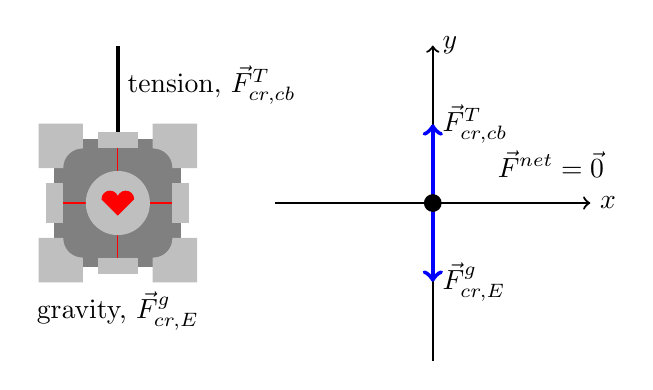
\begin{tikzpicture}
			\begin{scope}[shift={(-2,0)}]
				%\draw[thick] (-1,1) -- (1,1) -- (1,-1) -- (-1,-1) -- cycle;
				\filldraw[gray] (-0.8,0.8) -- (0.8,0.8) -- (0.8,-0.8) -- (-0.8,-0.8) -- cycle;
				\filldraw[lightgray] (-1,1) -- (-0.45,1) -- (-0.45,0.7) arc (90:180:0.25) -- (-1,0.45) -- cycle;
				\filldraw[lightgray,rotate=90] (-1,1) -- (-0.45,1) -- (-0.45,0.7) arc (90:180:0.25) -- (-1,0.45) -- cycle;
				\filldraw[lightgray,rotate=180] (-1,1) -- (-0.45,1) -- (-0.45,0.7) arc (90:180:0.25) -- (-1,0.45) -- cycle;
				\filldraw[lightgray,rotate=270] (-1,1) -- (-0.45,1) -- (-0.45,0.7) arc (90:180:0.25) -- (-1,0.45) -- cycle;
				\draw[red] (-0.8,0) -- (0.8,0);
				\draw[red] (0,-0.8) -- (0,0.8);
				\filldraw[lightgray] (-0.9,0.25) -- (-0.7,0.25) -- (-0.7,-0.25) -- (-0.9,-0.25) -- cycle;
				\filldraw[lightgray,rotate=90] (-0.9,0.25) -- (-0.7,0.25) -- (-0.7,-0.25) -- (-0.9,-0.25) -- cycle;
				\filldraw[lightgray,rotate=180] (-0.9,0.25) -- (-0.7,0.25) -- (-0.7,-0.25) -- (-0.9,-0.25) -- cycle;
				\filldraw[lightgray,rotate=270] (-0.9,0.25) -- (-0.7,0.25) -- (-0.7,-0.25) -- (-0.9,-0.25) -- cycle;
				\filldraw[lightgray] (0,0) circle (0.4);
				\filldraw[red] (-0.2,0.05) arc (180:0:0.1) arc (180:0:0.1) -- (0,-0.15) -- cycle;
				\draw[ultra thick] (0,0.9) -- (0,2);
				\node[anchor=north] at (0,-1) {gravity, $\vec{F}^{g}_{cr,E}$};
				\node[anchor=west] at (0,1.5) {tension, $\vec{F}^{T}_{cr,cb}$};
			\end{scope}
			\FBDaxes{2,0}{0}{axes}
			\FBDvectorXY{axes}{0,1}{FT}
			\node[anchor=west] at (FTtip) {$\vec{F}^{T}_{cr,cb}$};
			\FBDvectorXY{axes}{0,-1}{FG}
			\node[anchor=west] at (FGtip) {$\vec{F}^{g}_{cr,E}$};
			\FBDdot{axes}
			\node at ($(axes) + (1.5,0.5)$) {$\vec{F}^{net}=\vec{0}$};
		\end{tikzpicture}
	\end{figure}
}
\ProblemSub{\Brick}{
	(b) A brick is falling from the roof a three-story building.
}
\Solution{\BrickFig}{
	\begin{figure}[h]
		\centering
		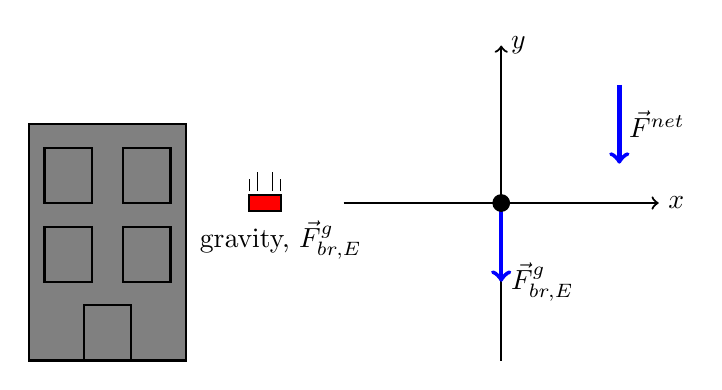
\begin{tikzpicture}
			\begin{scope}[shift={(-3,0)}]
				\filldraw[gray,draw=black,thick] (-1,-2) -- (1,-2) -- (1,1) -- (-1,1) -- cycle;
				\draw[thick] (-0.3,-2) -- (0.3,-2) -- (0.3,-1.3) -- (-0.3,-1.3) -- cycle;
				\draw[thick,shift={(0.5,1)}] (-0.3,-2) -- (0.3,-2) -- (0.3,-1.3) -- (-0.3,-1.3) -- cycle;
				\draw[thick,shift={(-0.5,1)}] (-0.3,-2) -- (0.3,-2) -- (0.3,-1.3) -- (-0.3,-1.3) -- cycle;
				\draw[thick,shift={(0.5,2)}] (-0.3,-2) -- (0.3,-2) -- (0.3,-1.3) -- (-0.3,-1.3) -- cycle;
				\draw[thick,shift={(-0.5,2)}] (-0.3,-2) -- (0.3,-2) -- (0.3,-1.3) -- (-0.3,-1.3) -- cycle;
			\end{scope}
			\filldraw[red,draw=black,thick,shift={(-1,0)}] (-0.2,-0.1) -- (0.2,-0.1) -- (0.2,0.1) -- (-0.2,0.1) -- cycle;
			\draw (-1.2,0.15) -- (-1.2,0.3);
			\draw (-0.8,0.15) -- (-0.8,0.3);
			\draw (-1.1,0.15) -- (-1.1,0.4);
			\draw (-0.9,0.15) -- (-0.9,0.4);
			\node[anchor=north] at (-0.8,-0.1) {gravity, $\vec{F}^{g}_{br,E}$};
			\FBDaxes{2,0}{0}{axes}
			\FBDvectorXY{axes}{0,-1}{FG}
			\node[anchor=west] at (FGtip) {$\vec{F}^{g}_{br,E}$};
			\FBDdot{axes}
			\FBDvectorXY{$(axes)+(1.5,1.5)$}{0,-1}{Fnet}
			\node[anchor=west] at ($(Fnettip) + (0,0.5)$) {$\vec{F}^{net}$};
		\end{tikzpicture}
	\end{figure}
}
\ProblemSub[34]{\PushBox}{
	(c) A girl is pushing a box across a rough horizontal floor at a steadily increasing speed.
}
\Solution{\PushBoxFig}{We will use the subscript $S$ (as in ``surface'') for the floor.
	
	\begin{figure}[h]
		\centering
		\begin{tikzpicture}
			\node at (-3.5,0) {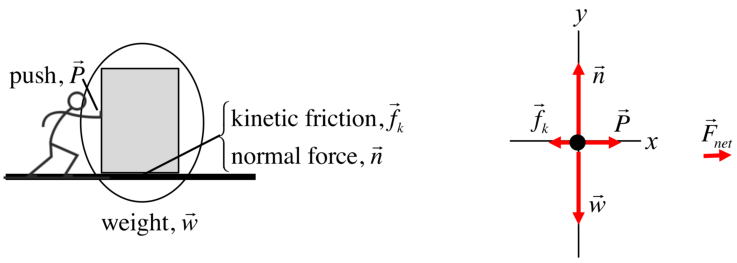
\includegraphics[trim={0 0 5cm 0},clip]{\FileDepth/Activities/Crate_Brick_Box_Car_FBDs/Girl_Pushing_the_Box_with_FBD}};
			\filldraw[white,shift={(-7.1,0.7)}] (0,0) rectangle (1.3,0.5);
			\node[anchor=south east] at (-5.7,0.7) {normal force, $\vec{F}^{N}_{BG}$};
			\filldraw[white,shift={(-5.6,-1.8)}] (0,0) rectangle (1.7,0.5);
			\node[anchor=south west] at (-5.6,-1.8) {gravity, $\vec{F}^{g}_{BE}$};
			\filldraw[white,shift={(-1,-0.6)}] (0,0) rectangle (0.5,0.5);
			\node[anchor=west] at (-1,-0.45) {$\vec{F}^{N}_{BS}$};
			\filldraw[white,shift={(-0.7,0)}] (0,0) rectangle (0.5,0.5);
			\node[anchor=west] at (-0.7,0.2) {$\vec{F}^{kf}_{BS}$};
			\FBDaxes{2.3,0}{0}{axes}
			\FBDvectorXY{axes}{0,-1.5}{FG}
			\node[anchor=west] at (FGtip) {$\vec{F}^{g}_{BE}$};
			\FBDvectorXY{axes}{0,1.5}{FNg}
			\node[anchor=west] at (FNgtip) {$\vec{F}^{N}_{BS}$};
			\FBDvectorXY{axes}{1,0}{FNp}
			\node[anchor=north] at (FNptip) {$\vec{F}^{N}_{BG}$};
			\FBDvectorXY{axes}{-0.5,0}{FK}
			\node[anchor=north] at (FKtip) {$\vec{F}^{kf}_{BS}$};
			\FBDvectorXY{$(axes)+(1.5,1)$}{0.5,0}{Fnet}
			\node[anchor=south] at (Fnettip) {$\vec{F}^{net}$};
			\FBDdot{axes}
		\end{tikzpicture}
	\end{figure}
}
\ProblemSub{\Brakes}{
	(d) You've slammed on your car brakes while going down a hill. The car is skidding to a stop.
}
\Solution{\BrakesFig}{
	\begin{figure}[h]
		\centering
		\begin{tikzpicture}
			\node at (-2.3,0) {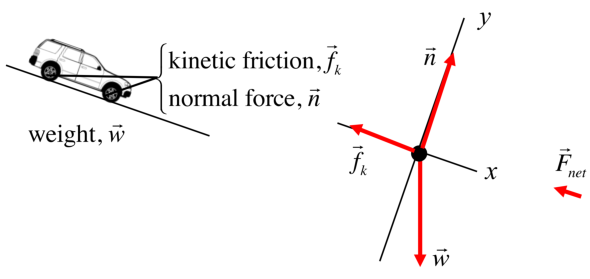
\includegraphics[trim={0 0 4.51cm 0},clip]{\FileDepth/Activities/Crate_Brick_Box_Car_FBDs/Car_Skidding_Downhill_with_FBD}};
			\filldraw[white,shift={(0.1,0.5)}] (0,0) rectangle (0.5,0.5);
			\node[anchor=west] at (0.4,1.3) {$\vec{F}^{kf}_{BS}$};
			\node[anchor=west] at (0.1,0.7) {$\vec{F}^{N}_{BS}$};
			\filldraw[white,shift={(-4.6,-0.2)}] (0,0) rectangle (1.7,0.5);
			\node[anchor=south west] at (-4.6,-0.2) {gravity, $\vec{F}^{g}_{BE}$};
			\FBDaxes{3,0}{-30}{axes}
			\FBDvectorMA{axes}{1.2}{150}{FK}
			\node[anchor=south] at (FKtip) {$\vec{F}^{kf}_{CS}$};
			\FBDvectorMA{axes}{1.5}{60}{FN}
			\node[anchor=west] at (FNtip) {$\vec{F}^{N}_{CS}$};
			\FBDvectorXY{axes}{0,-1.7}{FG}
			\node[anchor=north] at (FGtip) {$\vec{F}^{g}_{CE}$};
			\FBDvectorMA{$(axes)+(2,0)$}{0.4}{150}{Fnet}
			\node[anchor=south] at (Fnettip) {$\vec{F}^{net}$};
			\FBDdot{axes}
		\end{tikzpicture}
	\end{figure}
}
\end{document}